
\section{Background}
\label{sec:background}

In this section, we review the dragonfly topology, including the placement and routing policies examined in previous work. 

\subsection{Dragonfly Network}
\label{sec:network}
The dragonfly is a two-level hierarchical topology, consisting of several groups connected by all-to-all links. In each group, there could be $a$ routers connected via all-to-all local channels. For each router, there could be $p$ compute nodes attached to it via terminal links. The router has $h$ global channels used as intergroup connections through which it connected to other routers in different groups. Thus, the radix of each router is $k = a+h+p-1$. Different computing centers could choose different values for  $a$, $h$, $p$ when deploying their dragonfly network. The adoption of proper $a$, $h$, $p$ involves many factors such as system scale, building cost and workload characteristics. 

It is recommended that for the load balance purpose, a proper dragonfly configuration should follow $a=2p=2h$~\cite{kim-micro}. According to this configuration, the total number of groups, denoted as $g$ in the dragonfly network would be $g = a*h+1 $, the total number of compute nodes denoted as $N$ in the network would be $N = p*a*g $. An example dragonfly network is illustrated in Figure~\ref{fig:dragonfly-overview}. There are six routers in each group $(a=6)$, three compute nodes per router $(p=3)$, and three global channels per router $(h=3)$. This dragonfly network consists of 19 groups and 342 nodes in total.

\begin{figure}[h!] 
  \centering
  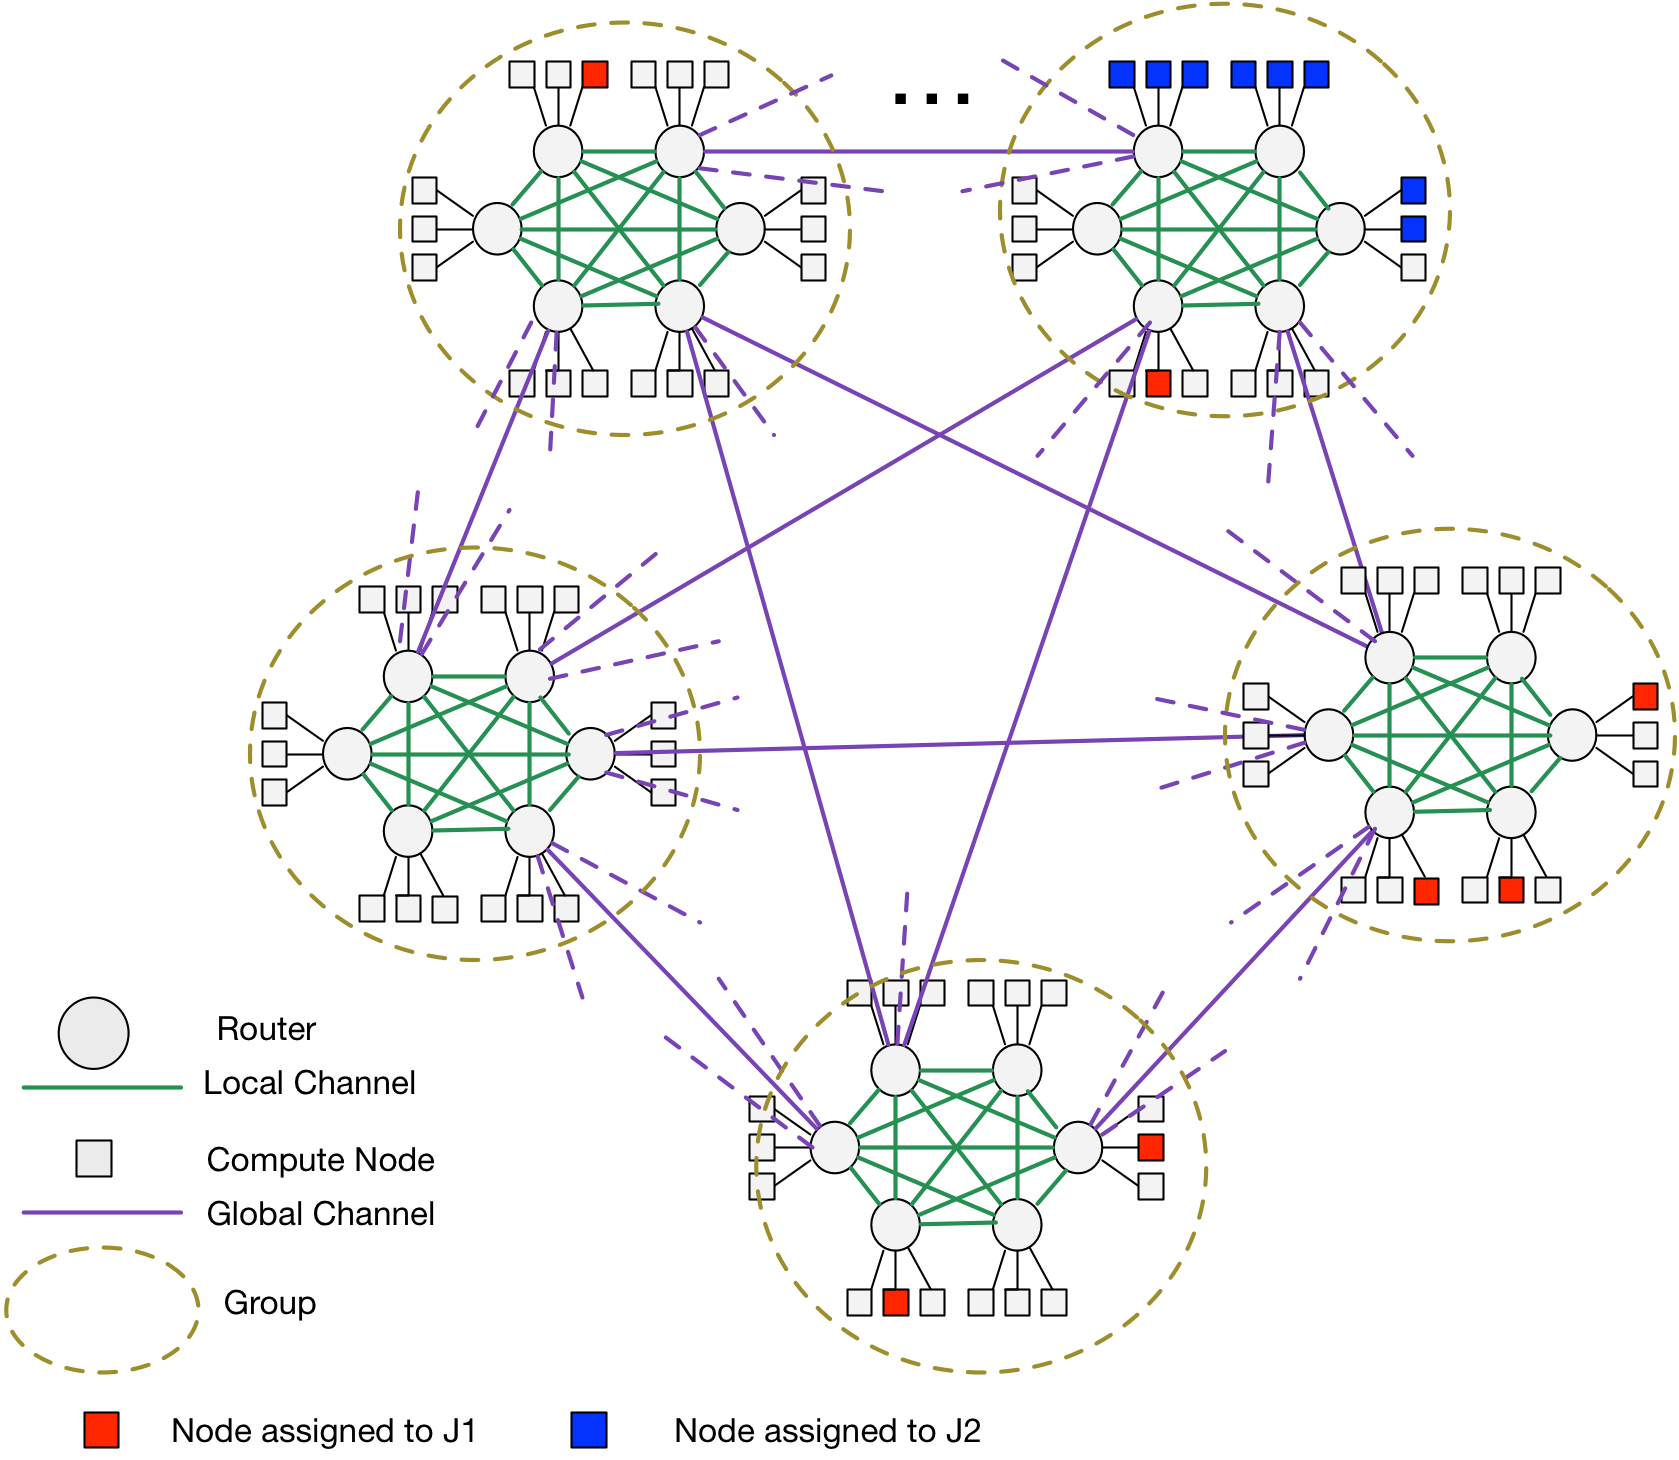
\includegraphics[width=0.48\textwidth]{dragonfly-overview}
  \caption{Five group slice of a 19-group dragonfly network. Job $J1$ is allocated using random placement, while Job $J2$ is allocated using contiguous placement.}
  \label{fig:dragonfly-overview}
\end{figure}


\subsection{Routing on Dragonfly}
\label{sec:routing-schemes}

The routing policy refers to the strategy adopted to route a message (a stream of packets) from the source router to the destination router. Previously studied routing policies for dragonfly network include minimal routing, adaptive routing~\cite{dally-dragonfly}, progressive adaptive routing~\cite{jiang} and some of their variations~\cite{won-prog-adaptive}. In this work we study three alternative routing policies considered by the community for dragonfly networks.

\textbf{Minimal:} In this policy, a message takes the minimal (shortest) path from the source router to the destination router. When there are multiple minimal paths between the source and destination, the message will be evenly divided among the paths. Minimal routing can guarantee the minimum hops the message takes from the source to the destination. However, it may result in congestion along the minimal paths. 

\textbf{Adaptive:} In this policy, the path a message takes will be adaptively chosen between minimal and non-minimal paths, depending on the congestion situation along those paths. For the non-minimal path, an intermediate router in a separate group will be randomly chosen. The message takes the intermediate router as a via point, connecting the source and destination router through two separate minimal paths. Adaptive routing can avoid hot-spots in the presence of congestion and collapse to minimal routing otherwise. 

\textbf{Progressive Adaptive:} In this policy, the decision to route minimally at each hop in the source group will be re-evaluated \TODO{packet granularity? flit granularity?}. Any decision to route non-minimally at source router or at a subsequent hop is permanent and will not be re-evaluated~\cite{jiang} \TODO{I thought PA does do re-evaluation?}. Progressive adaptive routing is capable of handling the case when a global channel is congested but the source router has not been informed yet~\cite{jiang}. The packet will take the non-minimal route only when the congestion is encountered. 

\subsection{Job Placement on Dragonfly}
\label{sec:placement-schemes}

For a parallel application requiring multiple compute nodes, job placement policy refers to the way of assigning the required number of nodes to the application by a system software such as batch scheduler~\cite{xu-cluster14}. In this work, we study two alternative placement policies considered by the community for dragonfly systems: 

\textbf{Random Placement:} In this policy, an application gets the required number of nodes randomly selected from all the available nodes in the system. As illustrated in Figure~\ref{fig:dragonfly-overview}, $J1$ gets random allocation in which nodes are attached to different routers in different groups. Routers may be shared by different applications and more routers are involved in serving each application when random placement is in use. Random placement can distribute the tasks of an application uniformly across the network to avoid the possible local congestion. However, random placement may cause congestion on global links.


\textbf{Contiguous Placement:} In this policy, the compute nodes are assigned to an application in a consecutive manner. The assignment first fills up a group, then crosses group boundaries and starts to fill the next group if necessary. As illustrated in Figure~\ref{fig:dragonfly-overview}, $J2$ gets eight nodes by contiguous placement. Contiguous placement confines the tasks of an application into the same group and uses minimum number of routers serving each application, which may result in local network congestion and increase the possibility of hot-spots. 
